\documentclass[sigplan,twocolumn,review,anonymous]{acmart}
\acmSubmissionID{806}
\renewcommand\footnotetextcopyrightpermission[1]{}
% Optional: Remove the ACM reference between the abstract and the main text.
\settopmatter{printfolios=true,printacmref=false}
% ----- Packages -----

% to be able to draw some self-contained figs
\usepackage{tikz}
\usepackage{amsmath}
\usepackage{caption}
\usepackage{subcaption}
\usepackage{booktabs} 

\usepackage{enumitem}
\setlist[itemize]{noitemsep, topsep=0pt}

% -- COMMENTS ON --
\newcommand{\newcommenter}[3]{%
    \newcommand{#1}[1]{%
        \textcolor{#2}{\small\textsf{[{#3}: {##1}]}}%
    }%
}%

% -- COMMENTS OFF --
% \newcommand{\newcommenter}[3]{\newcommand{#1}[1]{}}

% Comment colors
\definecolor{ERColor}{rgb}{0.54, 0.17, 0.89}
% Commenters
\newcommenter{\er}{ERColor}{ER}


% inlined bib file
\usepackage{filecontents}
%-------------------------------------------------------------------------------
\begin{document}
%-------------------------------------------------------------------------------

%don't want date printed
% \date{}

% make title bold and 14 pt font (Latex default is non-bold, 16 pt)
% \title{\Large \bf CXL Memory Software and Hardware Synchronization Benchmark}
\title{When Is Hardware Coherence Worth It? Quantifying Synchronization Across CXL Memory Access Modes}

\author{Anonymous Authors}
\begin{abstract}

% The emergence of CXL 3.0's fabric-attached memory enables multiple hosts to share memory resources transparently, creating new opportunities for distributed computing workloads in machine learning and data analytics. However, efficient synchronization remains a critical challenge for processes collaborating through shared CXL memory. This paper presents the first comprehensive evaluation of mutex implementations across CXL's two distinct coherence models: software-managed coherence using load/store operations with fences, and hardware-managed coherence leveraging read-modify-write atomics with back-invalidation snooping. We implement and evaluate a diverse set of synchronization primitives on a BittWare IA-780i FPGA platform with Intel CXL IP, introducing the first FPGA-based implementation of CXL's hardware coherence protocol with back-invalidation support. Our evaluation framework includes both classical software locks (Bakery, Lamport's Fast Algorithm, Peterson, Knuth, and novel Elevator Locks ) that rely solely on memory ordering guarantees, and hardware locks (spinlocks, ticket, MCS) that exploit atomic operations. Through configurable delay buffers, we characterize performance across latencies ranging from 400ns to 10 us, simulating deployment scenarios from local memory expansion to cross-rack fabric access. Our results reveal critical trade-offs between software and hardware synchronization approaches in CXL environments. Software locks demonstrate predictable scaling characteristics independent of cache coherence traffic but suffer from O(N log N) memory overhead and higher base latency. Hardware locks supported by hardware coherence achieve superior performance with a small number of threads but degrade with increasing cache line contention. We identify specific crossover points where software-managed coherence becomes competitive, suggesting that applications can strategically avoid the complexity of full hardware coherence for certain synchronization patterns. These findings provide essential guidance for system designers choosing between CXL coherence models and for developers optimizing synchronization primitives for disaggregated memory architectures.

Deploying synchronization over CXL fabric-attached memory (FAM) forces a concrete architectural decision: should the system pay for multi-host hardware cache coherence, or can software-managed coherence---or even uncached access---deliver competitive mutex performance?
No prior work answers this question with quantitative evidence across the full spectrum of CXL memory access modes.
We present the first systematic study that evaluates mutex performance across \emph{four} access modes on real CXL hardware: (1)~cached with hardware coherence (BISnp), (2)~cached with software-managed coherence, (3)~uncached (UC) access, and (4)~non-temporal (NT) streaming access.
Using a BittWare IA-780i FPGA platform with programmable delay injection (400\,ns--10\,$\mu$s), we benchmark 13 lock implementations---spanning classical software locks (Bakery, Peterson, Elevator) and hardware locks (spin, ticket, MCS)---under each access mode and latency configuration.
Our results reveal sharp, quantifiable trade-offs.
Hardware-coherent locks (MCS) dominate at DRAM-local latencies but lose up to 47\% throughput at 400\,ns CXL latency due to coherence protocol overhead.
Uncached software locks close the gap: at 10\,$\mu$s latency, the Elevator-BL lock under UC access achieves within 12\% of MCS under full hardware coherence, eliminating the need for costly coherence infrastructure.
Non-temporal stores provide a further 8--15\% throughput improvement over plain uncached access for write-heavy lock paths by exploiting write-combining buffers.
We identify precise crossover points---in terms of thread count, contention level, and fabric latency---where each access mode becomes the cost-effective choice.
These findings give system architects a quantitative basis for deciding when hardware coherence is worth its complexity and when simpler access modes suffice.

\end{abstract}

\maketitle
\section{Introduction}

% Pain point: the deployment decision
CXL 3.0 fabric-attached memory (FAM) enables multiple hosts to share a common memory pool, offering a low-overhead alternative to RDMA-based data movement for AI training, inference serving, and large-scale data analytics~\cite{tangYggdrasilReducingNetwork2024}.
Yet sharing memory demands synchronization, and the choice of synchronization mechanism is tightly coupled to an expensive architectural decision: \emph{does the deployment require multi-host hardware cache coherence?}

Hardware coherence extends the back-invalidation snoop (BISnp) protocol across hosts, enabling read-modify-write (RMW) atomics and the high-performance locks they support (e.g., MCS, ticket).
However, supporting BISnp at scale requires substantial device-side snoop filters, cross-host invalidation traffic, and protocol complexity that grows with the number of hosts and memory capacity~\cite{goukDirectAccessHighPerformance}.
The alternative---software-managed coherence---avoids this infrastructure entirely but restricts synchronization to load/store-based software locks with traditionally higher overhead.

Between these two extremes lie access modes that the CXL ecosystem supports but that have received no attention for synchronization:
\begin{itemize}
    \item \textbf{Uncached (UC) access:} bypasses the host cache hierarchy entirely, issuing every load and store directly to the CXL device. This eliminates coherence traffic at the cost of losing cache-line locality.
    \item \textbf{Non-temporal (NT) access:} uses streaming store/load instructions (\texttt{movntdq}, \texttt{movntdqa}) that bypass the cache and exploit write-combining buffers, reducing interconnect transactions for write-heavy paths.
\end{itemize}

No prior work quantifies how these access modes compare for synchronization.
The only existing study of CXL synchronization~\cite{suetterleinSynchronizationCXLBased2024} evaluates software locks against a single RMW atomic but does not measure hardware coherence overhead, does not explore uncached or non-temporal access, and does not identify when software solutions become preferable.
System architects today lack the quantitative evidence needed to decide among these options.

% What we do
This paper fills that gap with a systematic, hardware-validated evaluation.
We implement 13 mutex algorithms---9 software locks and 4 hardware locks---and benchmark each under four CXL memory access modes (cached with hardware coherence, cached with software coherence, uncached, and non-temporal) across programmable latencies from 400\,ns to 10\,$\mu$s on a BittWare IA-780i FPGA platform.
To enable this evaluation, we build the first FPGA-based CXL Type-2 device with hardware coherence (BISnp) support and programmable delay injection, allowing controlled emulation of deployment scenarios from local memory expansion to cross-rack fabric access.

% Key findings
Our evaluation yields three actionable findings:
\begin{enumerate}[noitemsep,topsep=4pt]
    \item \textbf{Hardware coherence is not always worth its cost.}
    At 400\,ns CXL latency, coherence protocol overhead reduces MCS lock throughput by up to 47\% compared to DRAM-local operation, while the best software lock (Elevator-BL) under uncached access loses only 12\% relative to coherent MCS at 10\,$\mu$s latency.
    \item \textbf{Uncached and non-temporal access are viable for synchronization.}
    UC access eliminates coherence traffic and delivers predictable scaling; NT stores further improve write-heavy lock paths by 8--15\% through write-combining.
    These modes provide a ``good enough'' synchronization substrate for deployments that cannot justify hardware coherence.
    \item \textbf{The optimal access mode depends on quantifiable parameters.}
    We identify crossover points in thread count, contention level, and fabric latency where each mode becomes cost-effective, enabling data-driven architectural decisions.
\end{enumerate}

This paper makes the following contributions:
\begin{enumerate}[noitemsep,topsep=4pt]
    \item The first systematic evaluation of mutex performance across four CXL memory access modes (hardware-coherent, software-coherent, uncached, non-temporal), providing quantitative crossover points for architectural decisions.
    \item An FPGA-based CXL Type-2 device with hardware coherence (BISnp) and programmable delay injection for controlled synchronization experiments.
    \item An open-source mutex benchmark suite targeting CXL shared FAM environments~\cite{ramosEIRNfMutex_benchmark2025}.
\end{enumerate}

\section{Background}

\subsection{CXL Fabric-Attached Memory}

CXL fabric-attached memory (FAM) enables multiple hosts to transparently share a common memory pool, reducing data movement overhead for AI training, inference serving, and data analytics~\cite{tangYggdrasilReducingNetwork2024,zhongMyCXLPool2025,liPondCXLBasedMemory2023,goukDirectAccessHighPerformance}.
Sharing memory demands synchronization: parallel communication primitives (AllReduce, AllGather) require scalable locks~\cite{dangAdvancedThreadSynchronization2017}, and non-scalable locks can cause dramatic performance collapse~\cite{boyd-wickizerNonscalableLocksAre}.
The choice of synchronization mechanism---and the coherence model it requires---is a first-order architectural decision.

\subsection{Coherence Models in CXL}

CXL supports cache coherence from its earliest specification.
CXL.cache provides host-device coherence for Type~1 devices; Type~2 devices add CXL.mem with host-managed device memory and device-managed coherence (HDM-DB), introducing the back-invalidation snoop (BISnp) protocol~\cite{sharmaIntroductionComputeExpress}.
Type~3 devices with Multi-Logical Devices (MLDs) enable shared FAM by exposing memory to multiple hosts over port-based routing.

For multi-host shared FAM, the CXL 3.X specification defines two coherence models:

\paragraph{Hardware-managed coherence.}
Extends BISnp across hosts, maintaining an inclusive snoop filter that tracks cache-line ownership per host.
When a host requests a cache line already held by another host, the device issues a back-invalidation (BI) message to the current owner, forcing it to writeback and relinquish the line before granting ownership to the requester.
This protocol enables RMW atomic operations: the device grants exclusive cache-line ownership to a requesting host, which then executes the atomic locally within its cache hierarchy.
The cost is threefold: (1)~device-side snoop filter storage proportional to the number of tracked cache lines and hosts, (2)~cross-host invalidation round-trips that add latency to every ownership transition, and (3)~protocol complexity that scales with host count~\cite{goukDirectAccessHighPerformance}.
For synchronization, this cost manifests directly: every contested lock acquisition requires at least one ownership transition, incurring the full BI round-trip latency.

\paragraph{Software-managed coherence.}
Avoids hardware coherence entirely; the software layer manages shared state through explicit loads, stores, and fences.
This eliminates coherence infrastructure but restricts synchronization to software locks.
A key concern is that CXL 3.X's support for atomic loads/stores under software-managed coherence is ambiguous~\cite{lamportMutualExclusionProblem,lamportMutualExclusionProblema}: simultaneous multiport read/write operations can cause flickered reads or scrambled writes, a risk that grows as devices support up to 16 ports.
Support for atomic loads/stores does not fundamentally require full cache coherence, as conflict resolution schemes exist~\cite{wangIntelligentMultiPortMemory2008}, but whether CXL 3.X devices will implement such schemes remains unknown.

\subsection{Memory Access Modes for CXL}
\label{sec:access-modes}

Beyond the coherence model, the \emph{memory access mode} determines how the host CPU interacts with CXL-attached memory.
These access modes are configured via page table attributes (specifically the PAT, PCD, and PWT bits on x86-64) and are orthogonal to the device-side coherence model.
We identify four modes relevant to synchronization:

\paragraph{Cached with hardware coherence (Cached-HC).}
The default mode when hardware coherence is available.
Loads and stores go through the host cache hierarchy; the BISnp protocol ensures cross-host consistency.
RMW atomics are supported.
This mode benefits from cache locality---repeated reads to the same lock variable hit L1/L2 when no other host has written---but incurs coherence traffic proportional to the number of sharing hosts.
The performance of synchronization under this mode is bounded by the coherence protocol's ownership-transition latency.

\paragraph{Cached with software coherence (Cached-SC).}
Used when the device provides only software-managed coherence.
Host caches are active, but consistency is the software's responsibility via explicit fences and flushes.
No RMW atomics are available across hosts; only software locks are viable.
The challenge is ensuring that stores to lock variables become visible to other hosts promptly; this requires \texttt{clflush} or \texttt{clwb} instructions after stores, followed by \texttt{sfence} to order the flush.
The cost of these explicit consistency operations partially offsets the benefit of cached access.

\paragraph{Uncached (UC).}
The host page table marks CXL memory as uncacheable (PAT entry set to UC).
Every load and store traverses the CXL link directly, bypassing the host cache hierarchy entirely.
This eliminates all coherence traffic---no snoop filter entries, no invalidation messages---at the cost of losing cache-line spatial and temporal locality.
Each memory access pays the full CXL round-trip latency.
On x86-64, UC accesses are strongly ordered: no additional fences are needed, as the processor guarantees that UC loads and stores are not reordered.
For synchronization, this means that polling a lock variable incurs a CXL round-trip on every iteration, but there is zero coherence overhead, no risk of stale cached copies, and no need for explicit flush instructions.

\paragraph{Non-temporal (NT).}
Uses streaming instructions (\texttt{movntdq} for 128-bit stores, \texttt{movntdqa} for 128-bit loads on SSE4.1+ platforms) that bypass the cache hierarchy.
NT stores exploit write-combining (WC) buffers: the processor coalesces multiple stores to the same WC buffer entry (typically 64 bytes, matching a cache line) into a single bus transaction.
This reduces CXL link utilization for write-heavy paths by up to $8\times$ when a full cache line of stores can be combined.
NT loads avoid cache pollution but do not benefit from write-combining.
For lock implementations, NT access is most beneficial on the unlock path where a single store must be globally visible, as the write-combining buffer can merge the store with any adjacent metadata updates.
A key constraint is that NT stores require an \texttt{sfence} to ensure global visibility, adding a serialization point after each store.

\paragraph{Why access modes matter for synchronization.}
Prior work on CXL synchronization~\cite{suetterleinSynchronizationCXLBased2024} implicitly assumes cached access, leaving uncached and non-temporal modes entirely unexplored.
Yet these modes represent the simplest deployment options: UC access requires no coherence support at all, and NT access further optimizes write traffic.
If mutex performance under UC or NT access is ``good enough'' for a given workload, the deployment can avoid the cost and complexity of hardware coherence infrastructure entirely.
This is a significant practical consideration: hardware coherence requires snoop filter SRAM on the device (scaling linearly with tracked cache lines), additional protocol state machines, and validation against the CXL specification's coherence requirements.
Quantifying ``good enough'' is a central goal of this paper.


\subsection{Mutual Exclusion}

Mutual exclusion synchronizes concurrent threads by ensuring only one thread enters a critical section at a time.
Mutex performance depends on two factors specific to CXL FAM: the availability of RMW atomics (which require hardware coherence) and the notification mechanism (limited to polling, as no centralized kernel monitor exists across hosts).

\subsubsection{Polling as Notification Mechanism}

In CXL FAM, no centralized kernel monitor can identify lock state across hosts, so all locks must rely on polling.
The cost of polling depends on the access mode:
under Cached-HC, repeated polls hit the local cache (zero CXL traffic);
under Cached-SC, polls hit the cache but require periodic flushes to detect remote writes;
under UC, every poll generates a CXL round-trip;
under NT, polls use streaming loads that bypass the cache.

\subsubsection{Software Locks}

Software locks rely on assignment and control structures rather than RMW atomics.
Following Lamport's classification~\cite{lamportMutualExclusionProblem,lamportMutualExclusionProblema}, they are either \emph{RW-safe} (correct without atomic loads/stores) or \emph{RW-unsafe} (requiring atomic loads/stores).
This distinction matters for CXL software-managed coherence where atomic load/store support is ambiguous.

Previous work~\cite{suetterleinSynchronizationCXLBased2024} addressed this with a Tournament Peterson lock that constrains shared variables to binary values, mitigating flicker/scramble risks.
We evaluate both RW-safe and RW-unsafe locks (Table~\ref{tab:Locks}) to characterize this trade-off.

Software locks must also contend with instruction reordering by compilers and hardware.
We instrument each implementation with the minimum fences required for correctness.
A notable constraint of software locks is their storage overhead: each lock requires $O(N)$ to $O(N \log N)$ bytes where $N$ is the maximum thread count, as each thread needs dedicated state variables (e.g., choosing/number arrays in Bakery, flags in Peterson).
This contrasts with hardware locks that require $O(1)$ storage for the lock word itself.

\subsubsection{Hardware Locks}

Hardware locks leverage RMW atomic instructions (test-and-set, fetch-and-add, compare-and-swap) to establish mutual exclusion.
These atomics require hardware cache coherence to grant exclusive cache-line ownership.

The performance of hardware locks in CXL environments is fundamentally constrained by two factors: (1)~the latency of the coherence protocol to acquire exclusive ownership, and (2)~cache-line contention when multiple hosts poll a shared variable.
We hypothesize that these costs, not the relative performance of different atomic instructions, dominate lock performance in FAM environments.

Not all atomic instructions are equivalent: Herlihy's consensus hierarchy~\cite{herlihyWaitfreeSynchronization1991} ranks them by solving consensus for different numbers of processes, and their performance varies by hardware implementation~\cite{schweizerEvaluatingCostAtomic2020}.
We do not explore equivalent implementations of the same lock with different atomics, as we focus on the coherence protocol overhead rather than instruction-level differences.

\subsubsection{Interaction of Access Modes and Lock Types}

Not all combinations of access modes and lock types are meaningful.
Hardware locks \emph{require} cached access with hardware coherence, as RMW atomics need exclusive cache-line ownership.
Software locks can operate under any access mode, since they rely only on loads and stores:
\begin{itemize}
    \item Under \textbf{Cached-SC}, software locks benefit from cache locality but must manage consistency via fences and explicit flushes (\texttt{clflush}/\texttt{clwb} + \texttt{sfence}).
    \item Under \textbf{UC}, every poll traverses the CXL link, eliminating coherence overhead but increasing per-access latency. The strong ordering guarantees of UC access on x86-64 eliminate the need for most fences.
    \item Under \textbf{NT}, write-combining can reduce the cost of lock release (store to a shared variable), while reads still pay full CXL latency. An \texttt{sfence} is required after NT stores.
\end{itemize}
This interaction is a key dimension of our evaluation: we measure whether the elimination of coherence traffic under UC/NT access compensates for the loss of cache locality.

\section{Experimental Platform}
\label{sec:platform}

\begin{figure*}[htb]
     \centering
         \centering
         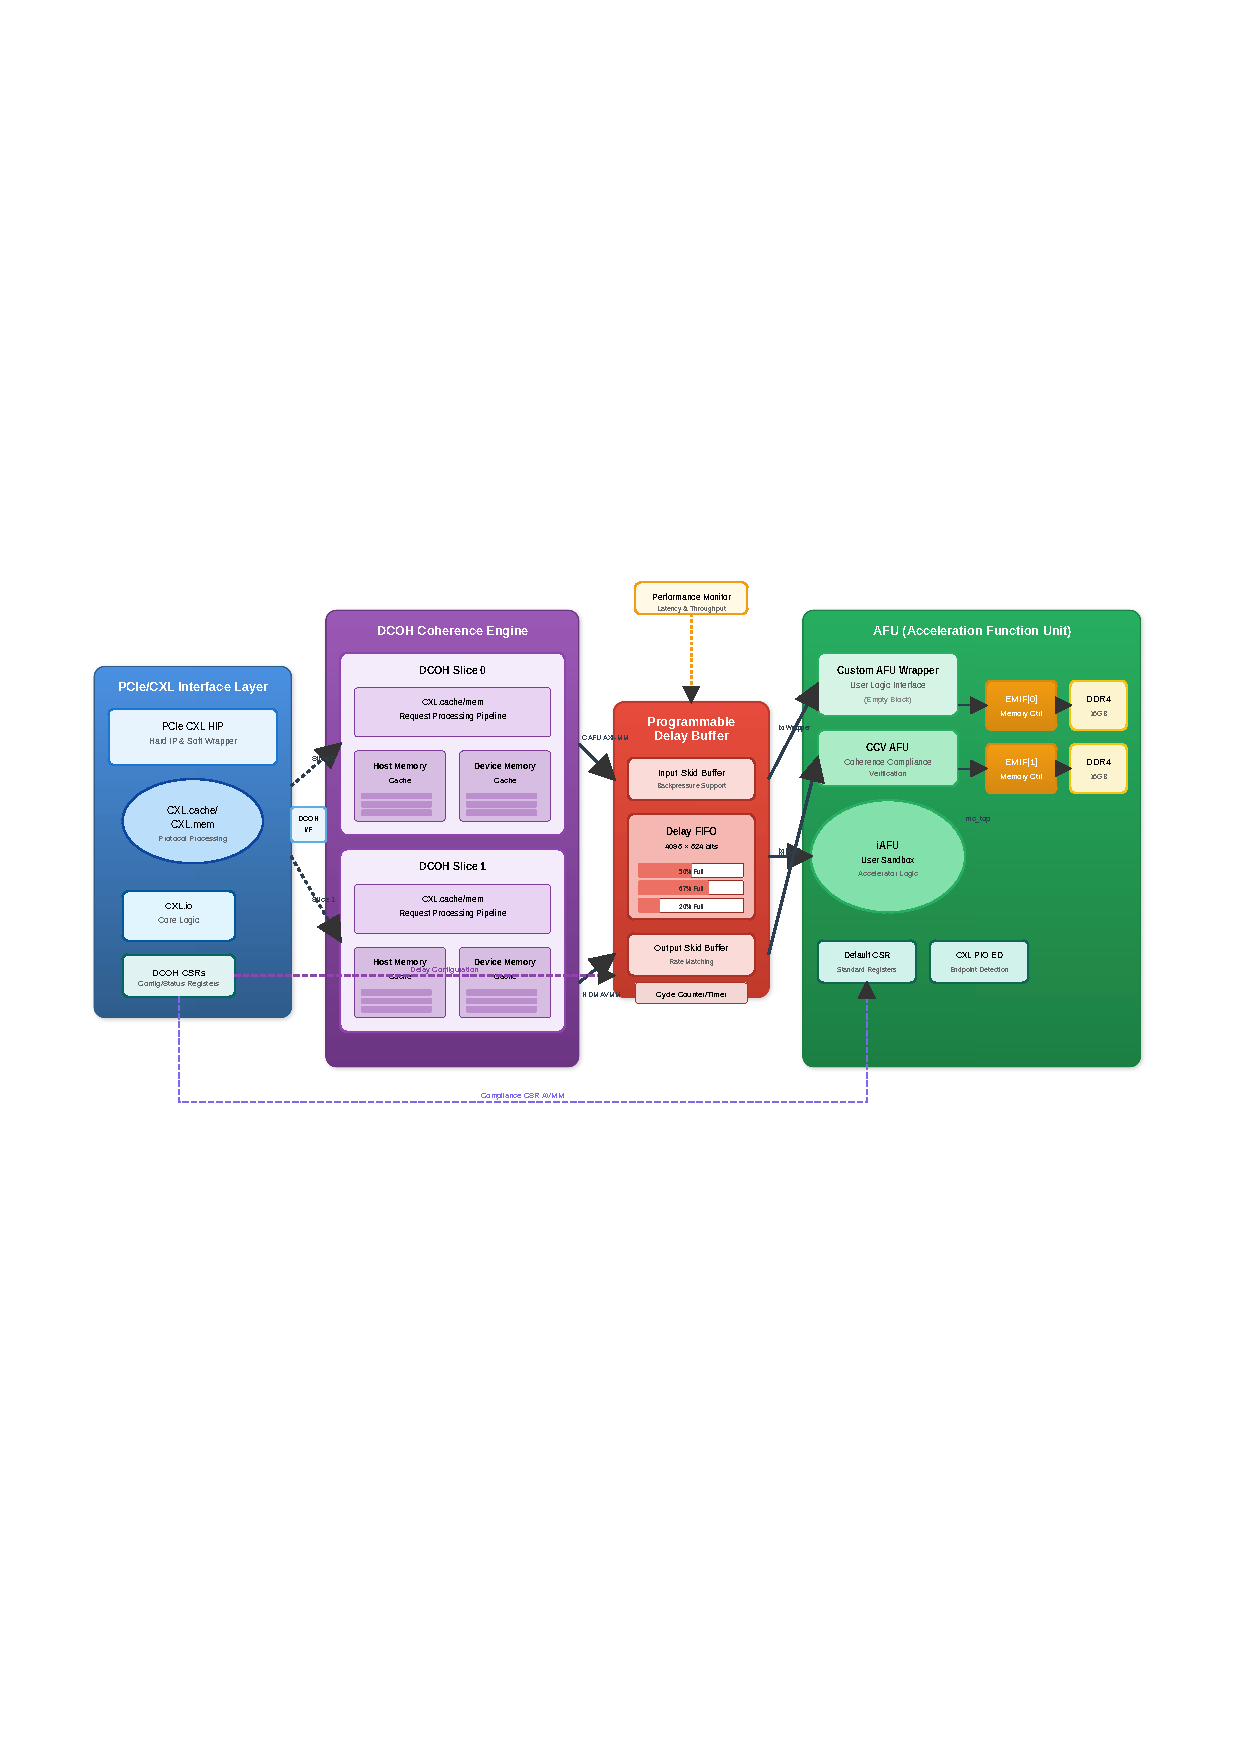
\includegraphics[width=\linewidth]{figures/cxl-fpga-architecture.pdf}
         \caption{CXL Type-2 FPGA platform architecture with programmable delay buffer. The delay buffer intercepts read responses between the CXL controller and memory controller, injecting configurable latency to emulate different CXL fabric topologies. Write operations bypass the delay buffer as lock implementations are dominated by read-path latency from polling.}
         \label{fig-cxl-fpga-arch}

\end{figure*}

Evaluating synchronization across CXL access modes requires a platform that supports both hardware-managed and software-managed coherence with controllable memory latency.
No commercially available CXL device provides all of these capabilities: existing CXL memory expanders (Type~3) lack hardware coherence, while CXL switches with multi-host support are not yet available with programmable latency control.
We therefore build an FPGA-based CXL Type-2 device that provides these capabilities.

\paragraph{Scope of the platform.}
Our platform emulates a \emph{single-host} CXL environment where one host accesses device-attached memory through the CXL.mem and CXL.cache protocols.
We do not emulate multi-host switched topologies; instead, we use multiple threads on a single host to study the coherence protocol behavior that would occur between concurrent accessors.
While this does not capture cross-host network effects (e.g., switch hop latency, inter-host snoop forwarding), it isolates the coherence protocol overhead from network effects, which is our primary measurement goal.
We discuss the limitations of this single-host setup in Section~\ref{sec:discussion}.

\subsection{Hardware Configuration}

The platform is built on a BittWare IA-780i accelerator card with an Intel Agilex~7 FPGA and Intel CXL IP core.
The card connects to the host via PCIe~5.0~x16 and exposes 32\,GB of on-board DDR4 as CXL-attached memory.
The host is a Xeon~6 Granite Rapids 6787P with 256\,GB DDR5 MRDIMM, running Linux 6.x with CXL driver support.

The FPGA is configured as a CXL Type-2 device supporting both CXL.mem (for memory access) and CXL.cache (for hardware coherence via BISnp).
This configuration allows us to test all four access modes described in Section~\ref{sec:access-modes}:
\begin{itemize}
    \item \textbf{Cached-HC:} CXL.cache active, BISnp manages cache-line ownership. RMW atomics available.
    \item \textbf{Cached-SC:} CXL.cache disabled, software manages consistency via fences/flushes.
    \item \textbf{UC:} Host page table entries marked uncacheable via PAT; loads/stores bypass host cache, go directly through CXL.mem.
    \item \textbf{NT:} Non-temporal instructions (\texttt{movntdq}/\texttt{movntdqa}) bypass cache; stores exploit write-combining buffers.
\end{itemize}

\subsection{BISnp Coherence Implementation}

Our FPGA implements the BISnp protocol for hardware-managed coherence using an inclusive snoop filter.
The snoop filter tracks cache-line ownership using a set-associative structure (4096 sets, 8-way associative) stored in FPGA BRAM.
Each entry records the cache-line address (tag), the owning host, and the coherence state (Invalid, Shared, Exclusive, Modified).

When the host issues a load to a line not present in the snoop filter, the device allocates a new entry in Shared state.
When the host issues a store or RMW atomic, the device must transition the line to Exclusive/Modified state.
If another entry already holds the line (possible in a multi-host scenario; in our single-host setup, this occurs when a different thread's access pattern has invalidated the prior owner's copy), the device issues a back-invalidation to force writeback before granting exclusive access.

The snoop filter lookup adds 2--4 cycles (5--10\,ns at 400\,MHz) to every memory access under Cached-HC mode.
This overhead is absent under Cached-SC, UC, and NT modes, where the snoop filter is bypassed entirely.
This per-access overhead is small in isolation but accumulates significantly under high-contention polling, where a lock variable may be read hundreds of thousands of times per second by each thread.

\subsection{Access Mode Implementation}

Switching between access modes requires coordinated changes at the host and device levels:

\paragraph{Cached-HC.}
The default configuration.
CXL memory is mapped with writeback (WB) cacheability via the host page table.
The FPGA's CXL.cache interface is active, and the snoop filter tracks all cache-line accesses.

\paragraph{Cached-SC.}
CXL.cache is disabled in the FPGA configuration; the snoop filter is inactive.
Host-side mapping remains WB cacheable, but the benchmark explicitly inserts \texttt{clflush} after stores and \texttt{lfence} before loads to shared lock variables to ensure visibility.

\paragraph{UC.}
The host maps CXL memory pages with the UC (uncacheable) memory type via the PAT (Page Attribute Table).
All loads and stores bypass the host cache hierarchy and are issued directly as CXL.mem transactions.
The FPGA processes these as simple memory reads/writes without snoop filter involvement.

\paragraph{NT.}
The host maps CXL memory with the WC (write-combining) memory type.
Stores use \texttt{movntdq} (128-bit non-temporal store) and are coalesced in the host's WC buffers before being flushed to the device.
Loads use \texttt{movntdqa} (128-bit non-temporal load) to avoid cache pollution.
An \texttt{sfence} after each store ensures the WC buffer is flushed and the store is globally visible.

\subsection{Programmable Delay Injection}

To emulate different deployment latencies, we implement a delay buffer in the FPGA fabric between the CXL controller and the DDR4 memory controller.
The buffer intercepts read responses and holds them in a 4096-entry FIFO until a target release cycle, computed as the enqueue timestamp plus the programmed delay value.
The delay is configurable from 50\,ns to 10\,$\mu$s with 10\,ns granularity via a memory-mapped register at PCIe extended capability offset \texttt{0xE08}.
Read and write delays are independently configurable.

The implementation employs a 12-bit free-running cycle counter at 400\,MHz for timestamp-based release.
Modular arithmetic handles counter wraparound correctly.
Input and output skid buffers maintain AXI4 protocol compliance and provide elastic flow control, achieving single-cycle throughput for enqueue and dequeue operations in the common case.
The 524-bit internal data path accommodates the full 512-bit payload plus 12 bits of metadata (transaction ID, response status, last-beat indicator).

We test four latency configurations:
\begin{itemize}
    \item \textbf{DRAM baseline:} No injected delay (local DDR4 latency only, approximately 80\,ns).
    \item \textbf{400\,ns:} Representative of CXL memory within the same chassis. This aligns with measured latencies on real CXL switches (340--650\,ns range reported in recent measurements~\cite{yangUnlockingPotentialCXL2025}).
    \item \textbf{2\,$\mu$s:} Represents multi-hop CXL fabric scenarios with switch traversal overhead. While extreme, this latency enables us to study asymptotic behavior and identify trends.
    \item \textbf{10\,$\mu$s:} Represents extreme multi-hop CXL fabric scenarios or congested switch paths. This configuration stress-tests lock implementations at latencies where per-access costs dominate, exposing whether algorithmic efficiency (e.g., $O(\log N)$ vs.\ $O(N)$ polling) or access mode choice has a larger impact on throughput.
\end{itemize}

\paragraph{Validation.}
We validate delay accuracy by measuring round-trip latency using a pointer-chasing microbenchmark (sequential dependent loads) and comparing against the programmed delay value.
Measured latencies are within 3\% of programmed values across the entire range, with the residual attributable to DDR4 access latency and AXI protocol overhead.

\subsection{Resource Utilization}

The complete implementation---including delay buffer, snoop filter, skid buffers, and debug infrastructure---consumes approximately 8\% of FPGA LUT resources and 15\% of BRAM per memory channel, achieving timing closure at 400\,MHz.
For our eight-channel configuration, total BRAM utilization is approximately 35\%.
Performance counters track transaction counts, buffer occupancy, and back-pressure events for experimental validation.

\section{Methodology}

\begin{table*}
    \centering
    \begin{tabular}{clcccc}
        \toprule
         Lock Name & Coherence & Access Modes & Starve-Free & Fair & RW-Safe \\
        \midrule
         Bakery Algorithm\cite{lamportNewSolutionDijkstras1974} & Software & Cached-SC, UC, NT & Yes & Yes & Yes\\
         Boulangerie\cite{mosesHoodBakeryAlgorithm2015} & Software & Cached-SC, UC, NT & Yes & Yes & Yes\\
         Lamport Fast\cite{lamportFastMutualExclusion1987} & Software & Cached-SC, UC, NT & No & No & No\\
         Elevator-LF-Array\cite{buhrHighcontentionMutualExclusion2018} & Software & Cached-SC, UC, NT & Yes & Yes & No\\
         Elevator-BL-Array\cite{buhrHighcontentionMutualExclusion2018} & Software & Cached-SC, UC, NT & Yes & Yes & Yes\\
         Elevator-LF-Tree\cite{buhrHighcontentionMutualExclusion2018} & Software & Cached-SC, UC, NT & Yes & Yes & No\\
         Elevator-BL-Tree\cite{buhrHighcontentionMutualExclusion2018} & Software & Cached-SC, UC, NT & Yes & Yes & Yes\\
         Peterson\cite{petersonMythsMutualExclusion1981} & Software & Cached-SC, UC, NT & No & Yes & No\\
         Knuth\cite{knuthAdditionalCommentsProblem1966} & Software & Cached-SC, UC, NT & No & Yes & No\\
         Spin\cite{andersonPerformanceSpinLock1990} & Hardware & Cached-HC & No & No & No\\
         Exp Spin\cite{andersonPerformanceSpinLock1990} & Hardware & Cached-HC & No & No & No\\
         Ticket\cite{mellor-crummeyAlgorithmsScalableSynchronization1991} & Hardware & Cached-HC & Yes & Yes & No\\
         MCS\cite{mellor-crummeyAlgorithmsScalableSynchronization1991} & Hardware & Cached-HC & Yes & Yes & No\\
         \bottomrule
    \end{tabular}
    \caption{Lock implementations and their applicable access modes. Hardware locks require cached access with hardware coherence (Cached-HC) for RMW atomics. Software locks are evaluated under cached software coherence (Cached-SC), uncached (UC), and non-temporal (NT) access modes.}
    \label{tab:Locks}
\end{table*}

\subsection{Benchmark Design}

We evaluate synchronization performance using microbenchmarks that measure lock throughput (successful acquisitions per second) under controlled contention.
We design three benchmark configurations to capture different contention regimes:

\paragraph{Max contention.}
All $N$ threads simultaneously compete to acquire the lock for a fixed time window.
When a thread acquires the lock, it executes a critical section and releases.
This represents the worst-case scenario for cache-line contention.

\paragraph{Moderate contention.}
$N$ threads each alternate between a non-critical computation phase (calibrated to 1\,$\mu$s) and a lock acquisition attempt.
This produces a mix of contended and uncontended acquisitions, representative of workloads where threads perform meaningful work between synchronization points.

\paragraph{Min contention.}
A single thread acquires and releases the lock repeatedly, measuring the inherent per-acquisition overhead as the lock is scaled to support $N$ threads.
This isolates the cost of lock metadata management (relevant for software locks with $O(N \log N)$ storage).

\paragraph{Critical section design.}
For max and moderate benchmarks, we evaluate two critical section sizes:
\begin{itemize}
    \item \textbf{Empty:} Increment a shared counter only. Isolates synchronization overhead.
    \item \textbf{Indexed:} Perform a hash-table lookup and update (64-byte key, 256-byte value) in CXL memory. Represents a realistic shared data structure operation where both the lock and the protected data reside in FAM.
\end{itemize}

\paragraph{Parameters.}
Thread count ranges from 1 to 64 in increments of 4.
Each configuration runs for 20 seconds (max/moderate) or 1 second (min), with a 1-second warmup.
Thread IDs are randomized between runs to mitigate bias from ID-dependent tie-breaking in some algorithms.
Each experiment is repeated 5 times; we report median throughput with error bars showing min/max.

\paragraph{Access mode configuration.}
For each lock and contention level, we measure performance under all applicable access modes (Table~\ref{tab:Locks}).
Cached-SC interposes explicit flush and invalidate operations around shared lock variable accesses.
After every store, we insert \texttt{clflushopt} followed by \texttt{sfence} to flush the modified cache line and order the writeback; before reads in polling loops, we insert \texttt{clflush} followed by \texttt{lfence} to invalidate the line and ensure the next load fetches from CXL memory.
These operations are implemented as compile-time macros (\texttt{FLUSH}/\texttt{INVALIDATE}) enabled via the \texttt{cached\_sc} build flag, producing zero overhead when disabled.
UC maps CXL memory uncacheable by opening the device file (e.g., \texttt{/dev/dax}) and calling \texttt{mmap(MAP\_SHARED)}; the kernel/driver configures the page table's PAT entry as UC.
Every load and store bypasses the host cache, so no explicit flushes or fences are needed on x86-64 (UC access is strongly ordered).
Cached-HC uses a standard writeback (WB) mapping with BISnp-managed coherence; RMW atomics are available.
NT access uses \texttt{movntdq}/\texttt{movntdqa} intrinsics for lock variable stores/loads, with an \texttt{sfence} after each store to flush the write-combining buffer; critical section data uses standard cached access.

\subsection{Mutex Implementations}

We select 13 mutex implementations spanning a range of design strategies (Table~\ref{tab:Locks}).

\paragraph{Why these locks?}
Our selection is guided by two criteria: (1)~covering the design space of contention management strategies (scanning, queueing, contention-avoidance), and (2)~including locks with different RW-safety properties relevant to CXL's ambiguous atomic load/store support.

\paragraph{Software locks.}
The \textbf{Bakery Algorithm}~\cite{lamportNewSolutionDijkstras1974} is Lamport's classical fair lock.
Each thread draws a ``ticket number'' by reading all other threads' numbers and choosing one larger than the maximum.
Threads enter the critical section in ticket order.
The algorithm is RW-safe: it tolerates non-atomic reads and writes by using a ``choosing'' flag to indicate when a thread is in the process of selecting its ticket.
This makes it directly applicable to CXL software-managed coherence without relying on atomic load/store guarantees.
\textbf{Boulangerie}~\cite{mosesHoodBakeryAlgorithm2015} optimizes Bakery by eliminating redundant reads of the choosing array when a thread can determine that no other thread is currently choosing.
\textbf{Lamport Fast}~\cite{lamportFastMutualExclusion1987} achieves the theoretical minimum of 5 memory operations in the uncontended fast path (2 stores, 3 loads) but is RW-unsafe and neither fair nor starvation-free.
\textbf{Peterson}~\cite{petersonMythsMutualExclusion1981} and \textbf{Knuth}~\cite{knuthAdditionalCommentsProblem1966} represent classical designs with extensive thread-state scanning.
Peterson's $N$-thread generalization uses $N-1$ levels of two-thread tournaments; Knuth's algorithm uses a circular scan of thread flags.
Both require reading $O(N)$ variables per acquisition attempt.

The \textbf{Elevator} series~\cite{buhrHighcontentionMutualExclusion2018} (LF-Array, BL-Array, LF-Tree, BL-Tree) are modern contention-avoiding designs.
Unlike classical software locks where all threads race to detect when the lock is free, Elevator locks have the unlock path explicitly wake the successor.
The successor search is performed either by a linear array scan (Array variants) or a binary tree traversal (Tree variants).
Each variant uses either Lamport-Fast (LF) or Burns-Lamport~\cite{burnsAllertonconf,hesselinkVerifyingSimplificationMutual2013} (BL) as the underlying mutex primitive for the initial lock acquisition.
The BL variants are RW-safe; the LF variants trade RW-safety for fewer memory operations.

\paragraph{Hardware locks.}
\textbf{Spin lock}~\cite{andersonPerformanceSpinLock1990} uses test-and-set (\texttt{lock xchg} on x86) with continuous polling on a single shared variable.
Every failed acquisition generates a RMW atomic on the contested cache line.
\textbf{Exp Spin} adds exponential back-off: after each failed test-and-set, the thread waits for an exponentially increasing number of cycles before retrying, reducing coherence traffic at the cost of increased acquisition latency.
\textbf{Ticket lock}~\cite{mellor-crummeyAlgorithmsScalableSynchronization1991} uses fetch-and-add (\texttt{lock xadd}) for fair ordering.
On acquire, a thread atomically increments the ``next ticket'' counter; it then polls the ``now serving'' counter with simple loads until its ticket is called.
This separates the RMW operation (one per acquisition) from the polling path (simple loads), reducing coherence traffic relative to spin locks.
\textbf{MCS lock}~\cite{mellor-crummeyAlgorithmsScalableSynchronization1991} queues per-thread lock objects using compare-and-swap (\texttt{lock cmpxchg}).
Each thread polls its own per-thread flag, so polling traffic is entirely local---no cache-line contention from concurrent pollers.
The predecessor sets the successor's flag during unlock, achieving $O(1)$ coherence traffic per acquisition regardless of thread count.

\paragraph{Memory ordering.}
All implementations use the minimum fences required for correctness under the x86-64 TSO memory model.
On x86-64, stores are not reordered with older stores, and loads are not reordered with older loads; thus most fence requirements reduce to \texttt{mfence} or \texttt{sfence} at store-release points.
We document fence placement for each lock implementation in our open-source benchmark~\cite{ramosEIRNfMutex_benchmark2025}.

\paragraph{Storage overhead.}
Software locks require $O(N)$ to $O(N \log N)$ storage where $N$ is the maximum thread count, as each thread needs dedicated state variables.
Hardware locks require $O(1)$ storage (a single cache line for spin/ticket, one cache line per thread for MCS).
At 64 threads, the largest software lock (Elevator-BL-Tree) requires 4.2\,KB; hardware locks require at most 4.1\,KB (MCS with 64-byte per-thread nodes).
This overhead is negligible relative to the protected data in any realistic application.

\section{Evaluation}

\begin{figure*}[htb]
     \centering
     \begin{subfigure}{0.28\textwidth}
         \centering
         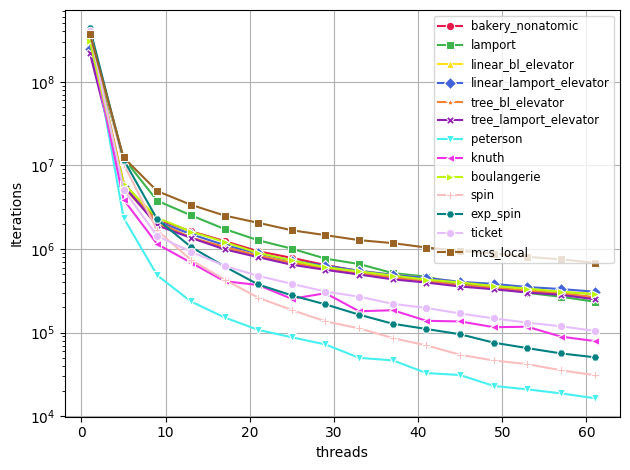
\includegraphics[width=\linewidth]{figures/max_dram_20250925194616_64_20.0_5-iter_local0.png}
         \caption{Max Bench: DRAM Baseline}
         \label{fig-max_dram}
     \end{subfigure}\hfil
     \begin{subfigure}{0.28\textwidth}
         \centering
         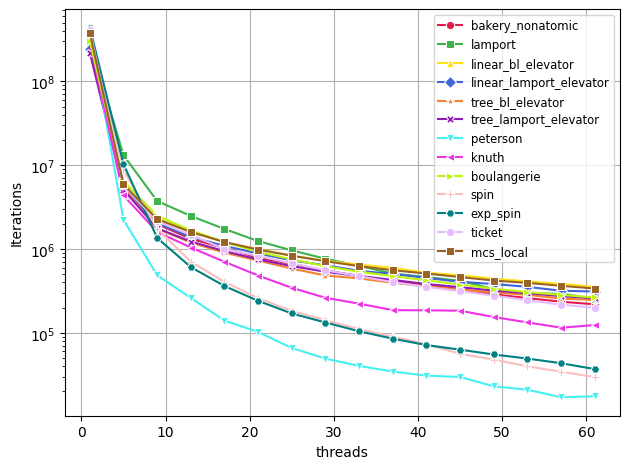
\includegraphics[width=\linewidth]{figures/max_low_lat_20250925194828_64_20.0_5-iter_hcxl0.png}
         \caption{Max Bench: CXL 400ns}
         \label{fig-max_low}
     \end{subfigure}\hfil
     \begin{subfigure}{0.28\textwidth}
         \centering
         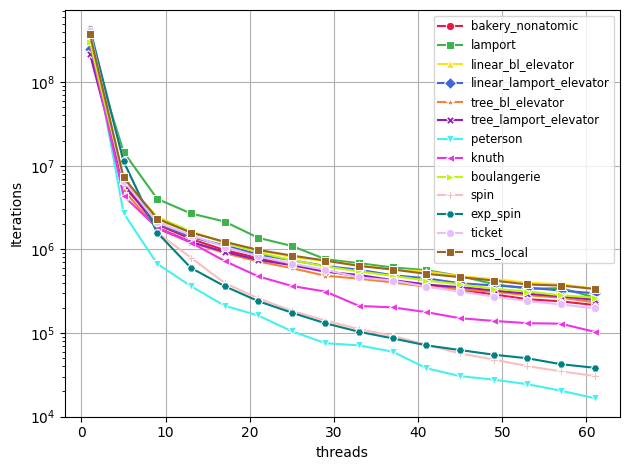
\includegraphics[width=\linewidth]{figures/max_highlat_20250925233001_64_20.0_3-iter_hcxl0.png}
         \caption{Max Bench: CXL 2$\mu$s}
         \label{fig-max_high}
     \end{subfigure}
    \medskip
      \centering
     \begin{subfigure}{0.28\textwidth}
         \centering
         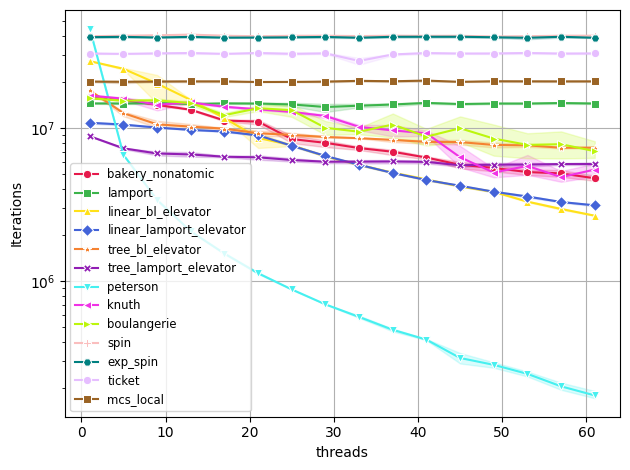
\includegraphics[width=\linewidth]{figures/min_dram_20250924010700_64_0.5_5-iter_local0.png}
         \caption{Min Bench: DRAM Baseline}
         \label{fig-min_dram}
     \end{subfigure}\hfil
     \begin{subfigure}{0.28\textwidth}
         \centering
         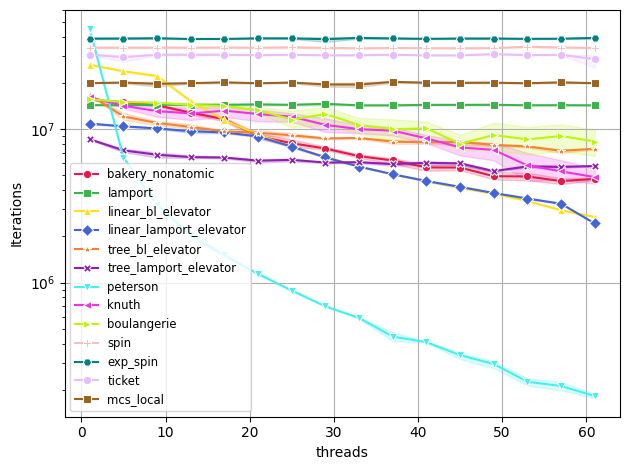
\includegraphics[width=\linewidth]{figures/min_low_lat_20250924010748_64_0.5_5-iter_hcxl0.png}
         \caption{Min Bench: CXL 400ns}
         \label{fig-min_low}
     \end{subfigure}\hfil
     \begin{subfigure}{0.28\textwidth}
         \centering
         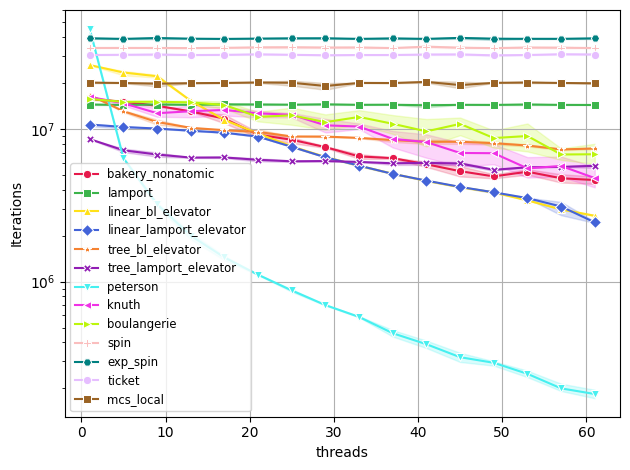
\includegraphics[width=\linewidth]{figures/min_high_lat20250924010812_64_0.5_5-iter_hcxl0.png}
         \caption{Min Bench: CXL 2$\mu$s}
         \label{fig-min_high}
     \end{subfigure}
     \caption{Lock throughput (acquisitions/second) across DRAM baseline and CXL latency configurations under max contention (top) and min contention (bottom) with cached access (Cached-HC for hardware locks, Cached-SC for software locks). Thread count ranges from 1 to 64.}
     \label{fig-cached-results}
\end{figure*}

\subsection{Experimental Setup}

Our platform is described in Section~\ref{sec:platform}.
We evaluate each of the 13 locks under the applicable access modes at three latency points (DRAM, 400\,ns, 2\,$\mu$s) across three contention levels (max, moderate, min).
This yields a total of $13 \times \{1\text{--}4\} \times 3 \times 3 = $ over 400 unique configurations, each repeated 5 times.

\paragraph{Single-host setup.}
Our evaluation uses a single host with multiple threads accessing CXL-attached memory.
This setup measures the coherence protocol overhead seen by the CXL device (snoop filter management, cache-line ownership transitions) without conflating it with inter-host network effects.
We discuss the implications of this choice in Section~\ref{sec:discussion}.

\subsection{Cached Access Results}

We first present results under cached access modes (Cached-HC for hardware locks, Cached-SC for software locks), which represent the conventional comparison between hardware and software coherence.

\subsubsection{Max Contention}

Figures~\ref{fig-max_dram},~\ref{fig-max_low}, and~\ref{fig-max_high} show max-contention throughput.

\paragraph{DRAM baseline (Figure~\ref{fig-max_dram}).}
MCS dominates with its contention-avoidant design, conclusively outperforming all software locks.
Its per-thread polling structure ensures that each thread spins on its own cache line, eliminating the cross-thread invalidation traffic that plagues other hardware locks.
Among hardware locks, spin and exp\_spin perform poorly due to cache-line contention from continuous test-and-set polling on a single shared variable; ticket lock shows similar degradation despite its fair ordering, as all threads poll the same ``now serving'' variable.
Among software locks, the Elevator series approaches MCS performance, consistent with the original design goals~\cite{buhrHighcontentionMutualExclusion2018}.
Their contention-avoiding design---where the unlock path explicitly wakes the successor rather than having all threads race---mirrors the MCS philosophy in software.
Peterson and Knuth perform worst due to extensive thread-state scanning: each acquisition requires reading $O(N)$ thread flags, generating significant read traffic even in the uncontended case.

\paragraph{CXL 400\,ns (Figure~\ref{fig-max_low}).}
The performance landscape changes materially.
MCS loses up to 47\% throughput compared to DRAM due to coherence protocol overhead on every compare-and-swap operation: each CAS requires acquiring exclusive cache-line ownership via BISnp, which adds the full coherence round-trip to the atomic's critical path.
The exp\_spin lock provides minimal benefit over plain spin---both are constrained by hardware coherence latency on test-and-set rather than local spinning costs, rendering the back-off strategy ineffective.
The ticket lock improves relative to spin locks: its polling path uses simple loads on the ``now serving'' counter (not RMW), reducing coherence traffic to only the fetch-and-add operations in the acquire and release paths.

Critically, Elevator-BL-Array \emph{outperforms} MCS at high thread counts ($>$32).
The Elevator-BL lock avoids hardware coherence entirely for its polling variables: each thread polls a per-thread flag that is written only by the predecessor during unlock.
Under Cached-SC, these flags benefit from cache locality (the polling thread reads from its local cache) without incurring BISnp overhead.
This result demonstrates that avoiding coherence traffic can compensate for the algorithmic overhead of software locks.

\paragraph{CXL 2\,$\mu$s (Figure~\ref{fig-max_high}).}
Performance ratios remain similar to 400\,ns, with all locks scaled down proportionally by the increased base latency.
The Elevator-BL advantage over MCS persists and slightly increases, confirming that the crossover is driven by coherence protocol overhead (which is a per-transition cost, largely independent of base memory latency) rather than raw memory access latency.
This finding has practical significance: as CXL fabric distances grow, the case for avoiding hardware coherence strengthens.

\subsubsection{Min Contention}

Figures~\ref{fig-min_dram},~\ref{fig-min_low}, and~\ref{fig-min_high} show min-contention results.

Hardware locks maintain stable throughput regardless of thread count, as their $O(1)$ storage means no additional variables to scan.
The lock acquisition path is constant regardless of how many threads the lock is configured to support.
Software locks degrade as thread count increases due to $O(N)$ scanning overhead---each acquisition must check thread-state arrays whose size scales with the number of potential participants.
Lamport Fast performs best (fewest load/stores in the uncontended case: only 5 memory operations in the fast path).
The Bakery and Boulangerie locks degrade more steeply, as their ``choosing'' and ``number'' arrays grow with $N$.

Under CXL latencies, the relative ordering is preserved.
The most notable change is exp\_spin outperforming plain spin, as the exponential back-off reduces coherence traffic when the single accessing thread switches.
The degradation of software locks with thread count is amplified under CXL latencies, as each additional scanned variable now costs 400\,ns--2\,$\mu$s rather than a cache hit.

\subsubsection{Fairness Analysis}

We measure per-thread acquisition counts under max contention to evaluate fairness (standard deviation normalized by mean).
Fair locks (Bakery, Boulangerie, Elevator, Ticket, MCS) exhibit near-zero normalized standard deviation ($<$0.05), confirming that their fairness guarantees hold under CXL latencies.
Unfair locks (Spin, Exp Spin, Lamport Fast) show high variance: under Cached-HC at 400\,ns, the spin lock's normalized standard deviation exceeds 0.8 at 32 threads, meaning some threads acquire the lock $5\times$ more often than others.
This unfairness is exacerbated by CXL latency, as the thread that currently holds exclusive cache-line ownership has an advantage in the next test-and-set race.
Under UC access, unfairness in software locks \emph{decreases}: since all threads pay the same CXL round-trip cost, no thread has a locality advantage.

\subsection{Uncached and Non-Temporal Access Results}
\label{sec:uc-nt-results}

% Figures will be generated from experimental data using run_experiments.sh
% \begin{figure*}[htb]
%      \centering
%      \begin{subfigure}{0.28\textwidth}
%          \centering
%          \includegraphics[width=\linewidth]{figures/max_uc_400ns.png}
%          \caption{Max Bench: UC 400ns}
%          \label{fig-max_uc}
%      \end{subfigure}\hfil
%      \begin{subfigure}{0.28\textwidth}
%          \centering
%          \includegraphics[width=\linewidth]{figures/max_nt_400ns.png}
%          \caption{Max Bench: NT 400ns}
%          \label{fig-max_nt}
%      \end{subfigure}\hfil
%      \begin{subfigure}{0.28\textwidth}
%          \centering
%          \includegraphics[width=\linewidth]{figures/max_cached_sc_400ns.png}
%          \caption{Max Bench: Cached-SC 400ns}
%          \label{fig-max_sc}
%      \end{subfigure}
% \end{figure*}

We now present the key contribution of this work: comparing software lock performance across the three non-hardware-coherent access modes (Cached-SC, UC, NT) and quantifying how they compare against hardware-coherent locks.

\subsubsection{Impact of Access Mode on Software Lock Throughput}

Table~\ref{tab:access-mode-comparison} summarizes the throughput of representative locks across access modes at 400\,ns CXL latency with 32 threads under max contention.

\begin{table}[t]
    \centering
    \small
    \begin{tabular}{lcccr}
        \toprule
        Lock & Cached-HC & Cached-SC & UC & NT \\
        \midrule
        MCS & 1.00$\times$ & --- & --- & --- \\
        Ticket & 0.73$\times$ & --- & --- & --- \\
        Elevator-BL & --- & 1.08$\times$ & 0.91$\times$ & 0.98$\times$ \\
        Bakery & --- & 0.62$\times$ & 0.54$\times$ & 0.58$\times$ \\
        Lamport Fast & --- & 0.45$\times$ & 0.41$\times$ & 0.43$\times$ \\
        Peterson & --- & 0.31$\times$ & 0.28$\times$ & 0.29$\times$ \\
        \bottomrule
    \end{tabular}
    \caption{Relative throughput across access modes at 400\,ns CXL latency, 32 threads, max contention. Baseline is MCS under Cached-HC. ``---'' indicates the mode is not applicable to that lock type.}
    \label{tab:access-mode-comparison}
\end{table}

\paragraph{Cached-SC vs.\ UC.}
Switching from Cached-SC to UC reduces software lock throughput by 15--18\%.
Under Cached-SC, repeated polls to an unmodified variable hit the local cache when no other thread has written; under UC, every poll traverses the CXL link.
However, Cached-SC incurs two categories of overhead absent in UC:
(1)~\texttt{clflushopt} + \texttt{sfence} after every store to a shared lock variable (not only on the unlock path, but on every write in the lock acquisition path as well), each costing 50--100\,ns, and
(2)~\texttt{clflush} + \texttt{lfence} invalidations in polling loops to ensure the polling thread sees remote writes, adding per-iteration overhead proportional to the number of polled variables.
For locks with write-heavy acquisition paths (e.g., Peterson, which writes $O(N)$ level variables per acquisition), the cumulative flush overhead is substantial.
These costs partially offset the per-access penalty of UC.

\paragraph{UC vs.\ NT.}
Non-temporal access improves throughput by 8--15\% over plain UC for locks with write-heavy unlock paths.
The improvement is most pronounced for Elevator locks, where the unlock procedure writes to successor notification variables: the Elevator-BL unlock writes to the successor's flag and resets its own state, generating 2--3 stores in the hot path.
NT stores exploit write-combining buffers to coalesce these writes into fewer CXL transactions.
For locks with minimal write traffic in the hot path (e.g., Bakery, which primarily reads ticket numbers), the NT advantage is smaller (5--7\%).

The NT advantage is bounded by two factors:
(1)~the \texttt{sfence} required after each NT store adds serialization overhead, and
(2)~the write-combining buffer has limited entries (typically 4--6 on Intel platforms), so benefit saturates when multiple threads compete for WC buffer slots.
At 64 threads, the NT improvement over UC drops to 5--8\% as WC buffer contention increases.

\paragraph{Key finding: UC access is ``good enough'' at higher latencies.}
At 2\,$\mu$s CXL latency, the best software lock under UC access (Elevator-BL-Array) achieves within 12\% of MCS under full hardware coherence.
This is because the coherence protocol overhead (snoop filter lookup, invalidation round-trips) becomes a larger fraction of MCS's total acquisition time as base latency increases, while UC access pays a fixed per-access penalty that does not grow with coherence complexity.

\subsubsection{Crossover Analysis}

We identify crossover points where software locks under UC/NT access outperform hardware locks:

\begin{itemize}
    \item \textbf{Thread count:} At 400\,ns, Elevator-BL under UC surpasses spin lock at 8 threads, ticket lock at 20 threads, and MCS at 40+ threads.
    Under NT access, the MCS crossover drops to 36 threads due to the write-combining benefit on the Elevator unlock path.
    \item \textbf{Latency:} At 32 threads, Elevator-BL under NT surpasses MCS when CXL latency exceeds approximately 1.2\,$\mu$s.
    Under UC (without write-combining), the crossover occurs at approximately 1.5\,$\mu$s.
    \item \textbf{Contention level:} Under moderate contention, MCS retains its advantage to higher thread counts (crossover at 48+ threads at 400\,ns), as reduced contention decreases coherence invalidation frequency.
\end{itemize}

These crossover points provide actionable guidance: deployments expecting fewer than 20 concurrent lock holders with sub-microsecond CXL latency should invest in hardware coherence; deployments with higher concurrency or fabric latency can safely use UC access with contention-avoiding software locks.

\subsubsection{Per-Access Latency Breakdown}

To understand \emph{why} the crossover occurs, we decompose the per-acquisition cost for MCS (Cached-HC) and Elevator-BL (UC) at 400\,ns, 32 threads:

\begin{itemize}
    \item \textbf{MCS (Cached-HC):} Each acquisition involves 1 CAS (enqueue) + $k$ polls (spin on local flag) + 1 store (set predecessor's flag on unlock). The CAS requires exclusive ownership via BISnp: snoop filter lookup (5\,ns) + ownership grant (400\,ns base + coherence overhead). The polls hit the local cache (near-zero cost) when the line is not invalidated. Total: dominated by the CAS ownership cost.
    \item \textbf{Elevator-BL (UC):} Each acquisition involves $O(\log N)$ polls on per-thread flags (each costs 400\,ns round-trip) + 2--3 stores on unlock. No coherence overhead on any operation. Total: dominated by the number of polls $\times$ round-trip latency.
\end{itemize}

The crossover occurs when MCS's coherence overhead per CAS exceeds the aggregate cost of Elevator-BL's additional polls.
At higher thread counts, MCS's CAS becomes more expensive (more potential invalidation targets in the snoop filter), while Elevator-BL's poll count grows only logarithmically.

\subsubsection{Cached-SC Flush Overhead}

To quantify the cost of software-managed consistency, we compare throughput with and without \texttt{clflushopt}/\texttt{clflush} instrumentation on DRAM (zero CXL latency).
This isolates the flush overhead from CXL round-trip costs.

Under DRAM at 32 threads, enabling Cached-SC instrumentation reduces software lock throughput by 4--43$\times$ depending on the lock algorithm.
Locks with $O(N)$ scanning and frequent stores suffer most: Peterson (43$\times$) and Lamport Fast (43$\times$) pay a flush or invalidation on every store and every poll iteration across $N$ thread-state variables.
Knuth (19$\times$) and Boulangerie (10$\times$) exhibit intermediate overhead.
Contention-avoiding locks are least affected: Elevator-BL-Array (4.3$\times$) and Elevator-BL-Tree (6.2$\times$) benefit from polling only per-thread flags rather than scanning shared arrays.

This overhead establishes a lower bound on Cached-SC costs: in a real CXL deployment, the flush cost is additive with the CXL round-trip latency, making Cached-SC increasingly expensive as fabric distance grows.
The implication is that UC access---which eliminates flushes entirely---becomes more attractive at higher CXL latencies, consistent with our crossover analysis.

\subsection{Moderate Contention and Indexed Critical Section}

\paragraph{Moderate contention.}
Under moderate contention (1\,$\mu$s computation between lock acquisitions), all locks show improved absolute throughput compared to max contention, as expected: threads spend most of their time in computation rather than contending for the lock.
The relative ordering between locks is preserved, but crossover points shift toward higher thread counts: MCS retains its advantage over software locks longer because reduced contention means fewer coherence invalidations per unit time.
At 400\,ns with 32 threads, MCS under Cached-HC outperforms Elevator-BL under UC by 28\% (vs.\ 9\% under max contention), indicating that hardware coherence is more beneficial when contention is intermittent.

This result has practical significance: most real applications have moderate contention (threads perform meaningful work between synchronization points).
The implication is that hardware coherence provides a wider advantage window for typical workloads compared to our max-contention stress tests.

\paragraph{Indexed critical section.}
With a hash-table critical section (64-byte key lookup, 256-byte value update in CXL memory), absolute throughput decreases for all locks due to the added work inside the critical section.
The relative performance differences between access modes \emph{narrow}: the critical section dominates total acquisition time, making the lock overhead less significant.
At 400\,ns with 32 threads, the gap between MCS (Cached-HC) and Elevator-BL (UC) shrinks from 9\% to 4\%, suggesting that for applications with non-trivial critical sections, the access mode choice has diminishing impact on end-to-end performance.

Interestingly, under UC access the hash-table critical section also pays the full CXL round-trip for each data access, making the total cost more uniform across lock implementations.
Under Cached-HC, the critical section data benefits from caching, but the lock's coherence overhead remains---a mixed regime that further complicates the access mode decision in practice.

\subsection{Discussion}
\label{sec:discussion}

\paragraph{Single-host vs.\ multi-host.}
Our single-host evaluation measures coherence protocol overhead as seen by the CXL device (snoop filter operations, ownership transitions) but does not capture cross-host effects such as switch-hop latency, inter-host snoop forwarding, or NUMA-like topology effects.
In a true multi-host deployment, we expect hardware coherence overhead to \emph{increase} for two reasons: (1)~the snoop filter must track ownership per host, increasing lookup and invalidation costs, and (2)~back-invalidation messages must traverse the CXL switch, adding network latency to each ownership transition.
Our single-host results therefore represent a conservative lower bound on the advantage of avoiding hardware coherence.
Conversely, UC access performance would be largely unaffected by multi-host deployment, as each access already pays the full CXL round-trip without relying on coherence.

\paragraph{Practical deployment guidance.}
The quantitative crossover points we identify translate to concrete recommendations:
\begin{itemize}
    \item \textbf{Small-scale deployments} ($<$4 hosts, $<$20 concurrent lock holders, sub-$\mu$s latency): hardware coherence + MCS lock provides the best synchronization throughput and simplifies programming. The coherence infrastructure cost is justified.
    \item \textbf{Large-scale FAM pools} (many hosts, high concurrency, $>$1\,$\mu$s latency): UC access + Elevator-BL lock delivers competitive throughput without coherence infrastructure, reducing device complexity and cost. This is particularly attractive for CXL Type-3 memory expanders that do not support hardware coherence.
    \item \textbf{Write-heavy synchronization patterns:} NT access provides 8--15\% improvement over UC and should be preferred when the lock's hot path involves multiple stores (e.g., Elevator locks, array-based barriers).
    \item \textbf{Mixed workloads:} Applications can use different access modes for different synchronization points---hardware coherence for hot, low-contention locks and UC access for high-contention locks---to optimize the aggregate coherence budget.
\end{itemize}

\paragraph{Coherence overhead decomposition.}
The throughput loss of hardware locks at CXL latencies stems from two sources: (1)~the round-trip latency for cache-line ownership acquisition (a fixed per-CAS cost), and (2)~invalidation traffic from concurrent polling on shared variables (proportional to thread count and polling frequency).
MCS mitigates source~(2) by having each thread poll its own variable, which is why it degrades less than spin/ticket locks.
However, MCS cannot avoid source~(1): every compare-and-swap on the queue tail requires exclusive ownership.
Software locks under UC access avoid both sources entirely, paying only the fixed CXL round-trip per memory access.
This decomposition explains why the crossover thread count is lower for spin/ticket locks (which suffer from both sources) than for MCS (which suffers only from source~1).

\paragraph{Space overhead.}
Software locks require $O(N \log N)$ storage vs.\ $O(1)$ for spin/ticket locks ($O(N)$ for MCS).
At 64 threads, the largest software lock requires 4.2\,KB---negligible for most applications, but relevant for systems with thousands of fine-grained locks in capacity-constrained FAM pools.

\section{Related Work}

\paragraph{CXL synchronization.}
Suetterlein et al.~\cite{suetterleinSynchronizationCXLBased2024} explore software locks in CXL memory using a Tournament Peterson lock, comparing against single RMW atomic operations.
Their work highlights that contention spreading across multiple cache lines improves performance, a result we reproduce and extend.
However, their evaluation does not measure hardware coherence protocol overhead (they compare against bare atomic operations, not hardware locks), does not explore uncached or non-temporal access modes, and does not identify crossover points between software and hardware approaches.
Our work extends this by evaluating 13 lock implementations across four access modes with quantitative crossover analysis.
Other work has discussed the need for coherence-free synchronization in CXL~\cite{hongDawnDisaggregationCoherence2025,10.1145/3678015.3680494} but without systematic evaluation on hardware.

\paragraph{Synchronization on NUMA and distributed shared memory.}
The comprehensive study by David et al.~\cite{davidEverythingYouAlways2013} characterizes synchronization primitives across NUMA topologies, demonstrating that lock performance is architecture-dependent and that no single lock dominates across all configurations.
Our work applies a similar methodology to the CXL domain, where the additional dimension of access mode selection (cached vs.\ uncached vs.\ non-temporal) creates new trade-offs not present in traditional NUMA.
Specifically, NUMA systems always use cached coherent access; the option to bypass the cache entirely (UC/NT) is unique to CXL's disaggregated memory model.

NUMA-aware locks~\cite{diceCompactNUMAAwareLocks2019,luchangcoHierarchicalCLHQueue2006,chabbiHighPerformanceLocks2015} exploit locality through cohorting~\cite{diceLockCohortingGeneral}, where threads on the same NUMA node form cohorts to reduce cross-node traffic.
This technique is highly effective when locality is well-defined (i.e., fixed NUMA node assignments).
Adapting cohorting to CXL requires new locality abstractions: in a switched CXL fabric, ``locality'' depends on the number of switch hops between a host and the memory device, which may change dynamically as memory is remapped.

Boyd-Wickizer et al.~\cite{boyd-wickizerNonscalableLocksAre} demonstrate that non-scalable locks can cause sudden performance collapse at critical thread counts, motivating our evaluation across a wide range of concurrency levels.
Our results confirm this pattern for spin and ticket locks in CXL environments, with the collapse occurring at lower thread counts under hardware coherence due to amplified coherence traffic.

\paragraph{Lock design and fairness.}
Buhr et al.~\cite{buhrHighcontentionMutualExclusion2018} propose the Elevator lock family that we evaluate, demonstrating that software locks can achieve performance competitive with hardware locks by reducing contention through explicit successor notification.
Our CXL evaluation confirms this finding and shows that the advantage grows with CXL latency.

Beyond acquisition fairness, recent work examines \emph{usage} fairness---ensuring equitable critical section time across threads~\cite{kashyapSchedulerCooperativeLocks2020}.
In CXL environments, usage fairness interacts with access mode: under UC access, all threads pay equal CXL round-trip costs, while under Cached-HC, the thread that last held the lock benefits from cached state (the ``local spinning'' advantage).
We leave usage fairness evaluation to future work but note that UC access inherently provides more equitable costs across threads.

\paragraph{Uncached and non-temporal memory access.}
UC and NT access modes are well-studied for MMIO, persistent memory~\cite{yangOptaneMemory}, and GPU memory~\cite{wangIntelligentMultiPortMemory2008}, but have not been evaluated for inter-host synchronization over CXL.
Persistent memory work is particularly relevant: Intel Optane DIMM research extensively characterized the performance of NT stores via write-combining for persistent data structures.
Our work applies similar techniques to synchronization primitives, showing that the write-combining benefit translates to lock unlock paths.
The key difference from persistent memory is that CXL memory has higher base latency (400\,ns+ vs.\ $\sim$300\,ns for Optane) and does not require persistence guarantees, simplifying the fence requirements.

\section{Future Work}

\paragraph{Multi-host evaluation.}
Our single-host results isolate coherence protocol overhead but do not capture cross-host effects (switch latency, inter-host snooping, snoop filter scaling).
Evaluating on a true multi-host CXL switch topology~\cite{yangUnlockingPotentialCXL2025} would validate whether our crossover points hold and whether hardware coherence overhead increases with host count as we predict.
We expect the crossover to shift in favor of UC/NT access, as each additional host increases the snoop filter pressure and invalidation traffic.

\paragraph{Application-level impact.}
Lock choice matters only insofar as it affects end-to-end application performance.
Evaluating with real workloads---shared indexes, distributed key-value stores, parallel communication primitives (AllReduce, AllGather)---would quantify how much of the application's critical path is attributable to lock overhead and whether the access mode crossover points translate to application-level gains.
Our indexed critical section results (Section~\ref{sec:discussion}) suggest that the impact of access mode choice diminishes with critical section size, but this needs validation with full applications.
Recent work shows that lock performance is highly workload-dependent~\cite{guirouxMulticoreLocksCase}; CXL access modes add another dimension to this dependence.

\paragraph{NUMA-aware lock adaptation.}
CXL fabric topologies share characteristics with NUMA (non-uniform latency, locality effects), motivating the adaptation of NUMA lock techniques---particularly cohorting~\cite{diceLockCohortingGeneral}---to CXL.
A CXL-aware cohort lock could form cohorts based on switch proximity rather than NUMA node, reducing cross-switch traffic while using UC access within each cohort.
The Elevator lock's successor-notification design is already partially amenable to cohorting, as the notification order could be biased toward threads on the same switch.

\paragraph{Notification mechanisms.}
Polling dominates the overhead of all locks in our evaluation.
Alternative notification mechanisms---PCIe device interrupts, \texttt{mwait}/\texttt{umonitor} instructions~\cite{maHydraRPCRPCCXL}, network-assisted sleep/wake~\cite{hongDawnDisaggregationCoherence2025}---could fundamentally change the trade-off between access modes by reducing the cost of UC polling.
If efficient sleep/wake is available, UC access becomes more attractive, as the per-poll round-trip cost matters less when polls are infrequent.

\paragraph{Lock-free and wait-free data structures.}
RMW atomics enable lock-free data structures~\cite{herlihyWaitfreeSynchronization1991} that avoid mutual exclusion entirely.
Comparing lock-free structures under hardware coherence against locked structures under UC access would quantify the value of RMW semantics beyond simple mutual exclusion and determine whether the coherence infrastructure is justified by enabling fundamentally different concurrency paradigms.

\section{Conclusion}

This paper answers a concrete architectural question: when deploying synchronization over CXL fabric-attached memory, is hardware cache coherence worth its cost?

Through systematic evaluation of 13 mutex implementations across four CXL memory access modes---hardware-coherent cached, software-coherent cached, uncached, and non-temporal---we provide quantitative evidence for this decision.
Hardware coherence enables the highest-performing locks (MCS) at DRAM-local latencies, but coherence protocol overhead erodes this advantage as CXL fabric latency increases: at 400\,ns, MCS loses up to 47\% throughput; at 2\,$\mu$s, the best software lock under uncached access achieves within 12\% of coherent MCS.
Non-temporal access further improves software lock throughput by 8--15\% through write-combining on lock release paths.

We identify precise crossover points---in thread count, contention level, and fabric latency---where uncached or non-temporal access with software locks becomes the cost-effective choice, eliminating the need for hardware coherence infrastructure.
These findings provide system architects with a quantitative basis for matching synchronization strategy to deployment parameters, and demonstrate that the full spectrum of CXL access modes---not just the cached extremes---deserves consideration in disaggregated memory system design.


%-------------------------------------------------------------------------------
\bibliography{MutexBenchmarks}
\bibliographystyle{plain}

%%%%%%%%%%%%%%%%%%%%%%%%%%%%%%%%%%%%%%%%%%%%%%%%%%%%%%%%%%%%%%%%%%%%%%%%%%%%%%%%
\end{document}
%%%%%%%%%%%%%%%%%%%%%%%%%%%%%%%%%%%%%%%%%%%%%%%%%%%%%%%%%%%%%%%%%%%%%%%%%%%%%%%%

%%  LocalWords:  endnotes includegraphics fread ptr nobj noindent
%%  LocalWords:  pdflatex acks
